\section{Results}
\label{sec:results}


\subsection{Effect of Conversation on Participants' Readiness to Quit Smoking}
\label{sec:result_readiness}

\begin{table}[phtb!]
  \centering
  \renewcommand{\arraystretch}{0.9}
  \setlength{\tabcolsep}{3pt}
  {
  \begin{tabular}{
  @{} p{0.23\linewidth}
  p{0.23\linewidth}
  p{0.23\linewidth}
  p{0.23\linewidth} @{}
  }
    \toprule
    \textbf{Average} &
    \textbf{Average} &
    \textbf{Average} &
    \textbf{Average $\Delta$}  \\

    \textbf{Before} &
    \textbf{After} &
    \textbf{1-Week} &
    \textbf{(1-Week }  \\

    \textbf{Conv} &
    \textbf{Conv} &
    \textbf{After} &
    \textbf{$-$ Before)}  \\

    \midrule\vspace{-4pt}\\[-8pt]

    \multicolumn{4}{@{}l}{\textit{\textbf{Importance}}} \\
    5.7 (2.6) & 6.3 (2.9) & 6.1 (2.7) &  0.5 (1.7)$^*$  \\

    \arrayrulecolor{gray!50}\midrule\vspace{-4pt}\\[-8pt]

    \multicolumn{4}{@{}l}{\textit{\textbf{Confidence}}} \\
    2.8 (2.0) & 4.6 (2.6) & 4.5 (2.7) & 1.7 (2.4)$^{**}$  \\

    \arrayrulecolor{gray!50}\midrule\vspace{-4pt}\\[-8pt]

    \multicolumn{4}{@{}l}{\textit{\textbf{Readiness}}} \\
    5.2 (2.8) & 5.9 (2.8) & 5.5 (3.0) &  0.3 (2.4)$^\dagger$ \\

    \arrayrulecolor{black}\bottomrule
  \end{tabular}}

  \caption{Average (SD) of Readiness Ruler Survey on Importance, Confidence, and Readiness to quit smoking. Statistical significance using Wilcoxon signed-rank test. $^*$: $p < 0.005$, $^{**}$: $p < 0.001$, $^\dagger$: $p = 0.22$.}

  \label{table:readiness_ruler}
\end{table}

Recall from Section~\ref{sec:evaluation} that the 106 human participants in the study completed the readiness ruler survey on three occasions: just before the conversation with the chatbot, just after it, and one week later. The primary measure of effectiveness is the difference in confidence from before the conversation to one week later, as this is the most predictive of downstream quitting success \citep{Gwaltney2009-wj}.
\textbf{Table~\ref{table:readiness_ruler}} presents data at those points in time for the three readiness rulers: importance, confidence, and readiness. It shows a significant increase in confidence of +1.7 on the ten-point scale.

As a point of reference, our previous work, \oldsysname \citep{info:doi/10.2196/49132}, which used a hybrid of scripted questions and LLM-generated reflections, reported an average change in confidence of +1.3. While that result is not directly comparable to the present one, both works recruited a similar number of low-confidence participants but at a different time and with a different starting average confidence.

We can also compare the week-later change in confidence to that achieved by human counsellors. \citet{rachelthesis} found that participants' confidence increased by +2.5 points after five MI sessions over a ten-week period.

\textbf{Figure~\ref{fig:confidence_change_dist}} presents the distribution of week-later changes in confidence scores. Notably, 28\% of  participants did not change their confidence level, but a substantial number (around 60\%) showed a positive change in confidence. Roughly 12\% decreased their confidence by 1-2 points, and a larger decrease was observed in 2\% of the participants.

\textbf{Table~\ref{table:readiness_ruler}} also shows that there was a significant change in the participants' view of the importance of quitting, with an average increase of +0.5, exhibiting the chatbot's effectiveness. The change in readiness was not statistically significant.

Finally, \textbf{Table~\ref{table:demographics_wise_conf}} in Appendix~\ref{appendix:demographics_wise_confidence} shows that baseline confidence levels and one-week changes varied by demographic group. Younger participants, for instance, started with a higher average confidence of 3.7 and saw a larger increase of +1.9 over the week.


\begin{figure}[!tphb]
\centering
  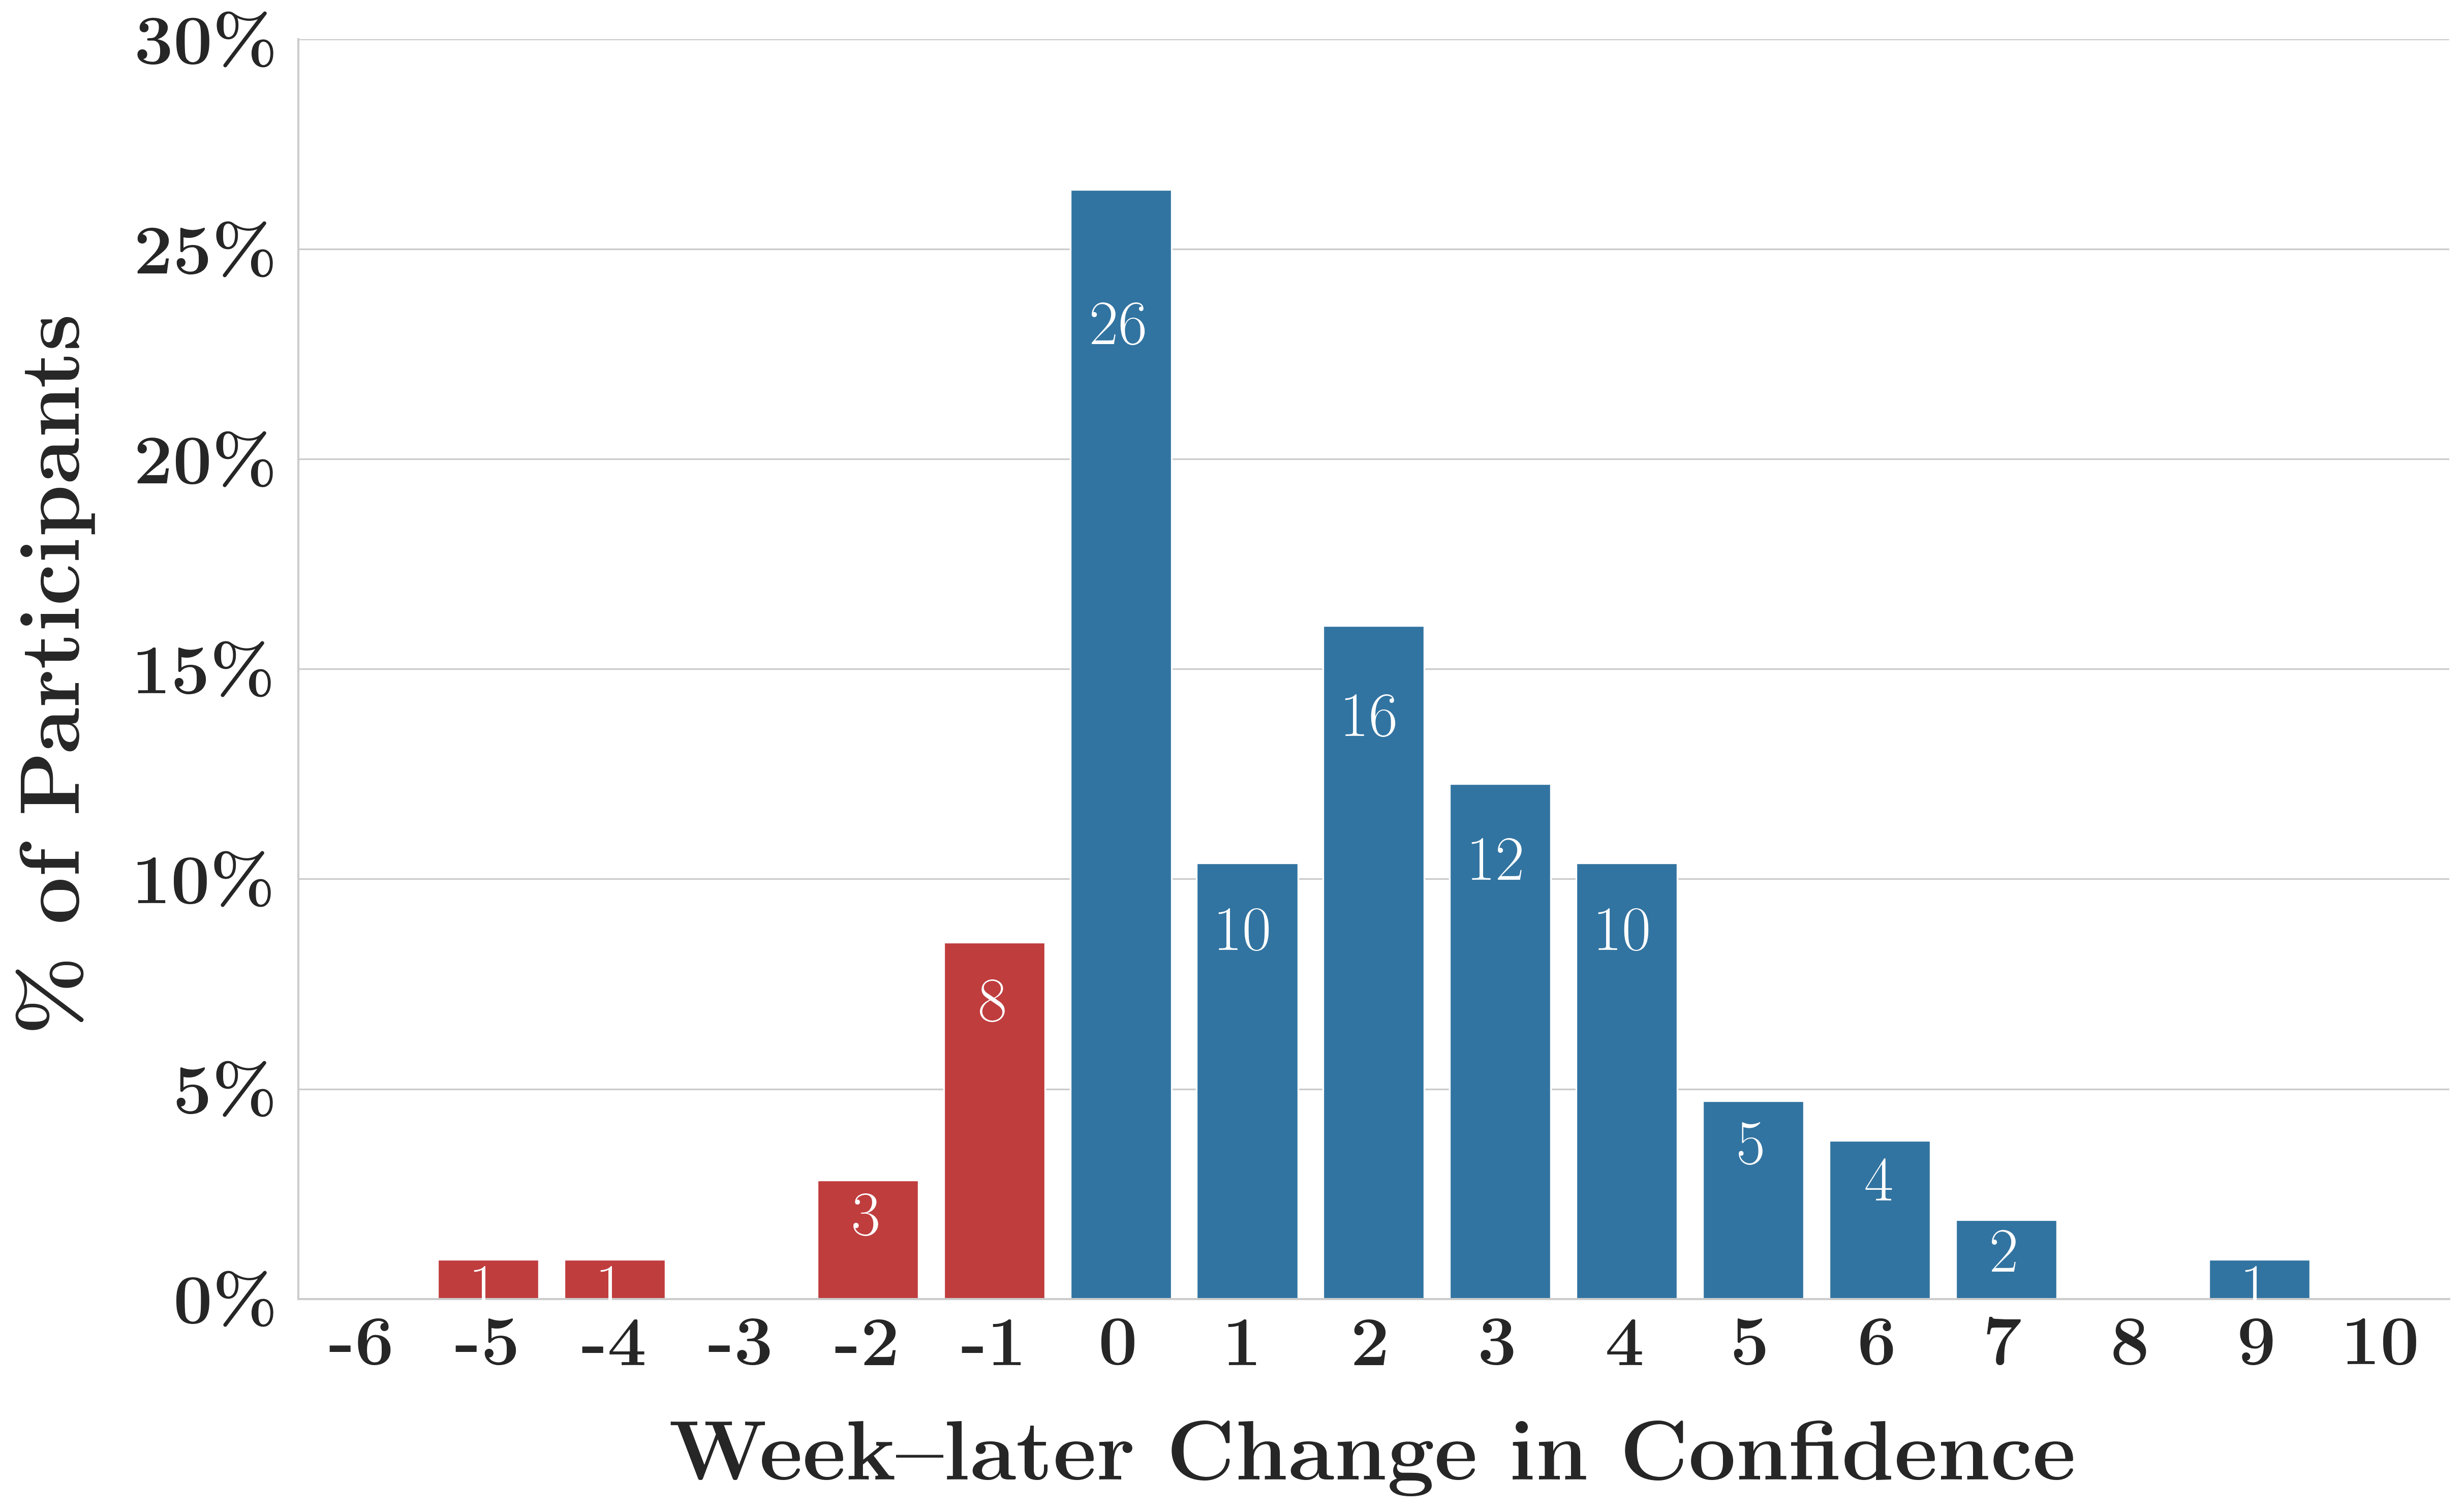
\includegraphics[width=\linewidth]{fig/2024-11-14-MIV6.3A-2024-11-22-MIV6.3A_ruler_deltas_delta_with_week_later_keep_high_conf_False_change.png}
  \caption {Distribution of Change in Confidence (1-Week Later $-$ Before Conversation).}
  \label{fig:confidence_change_dist}
\end{figure}

\begin{figure*}[htpb!]
    \centering
    \begin{subfigure}[b]{0.32\textwidth}
        \centering
        \captionsetup{justification=centering}
        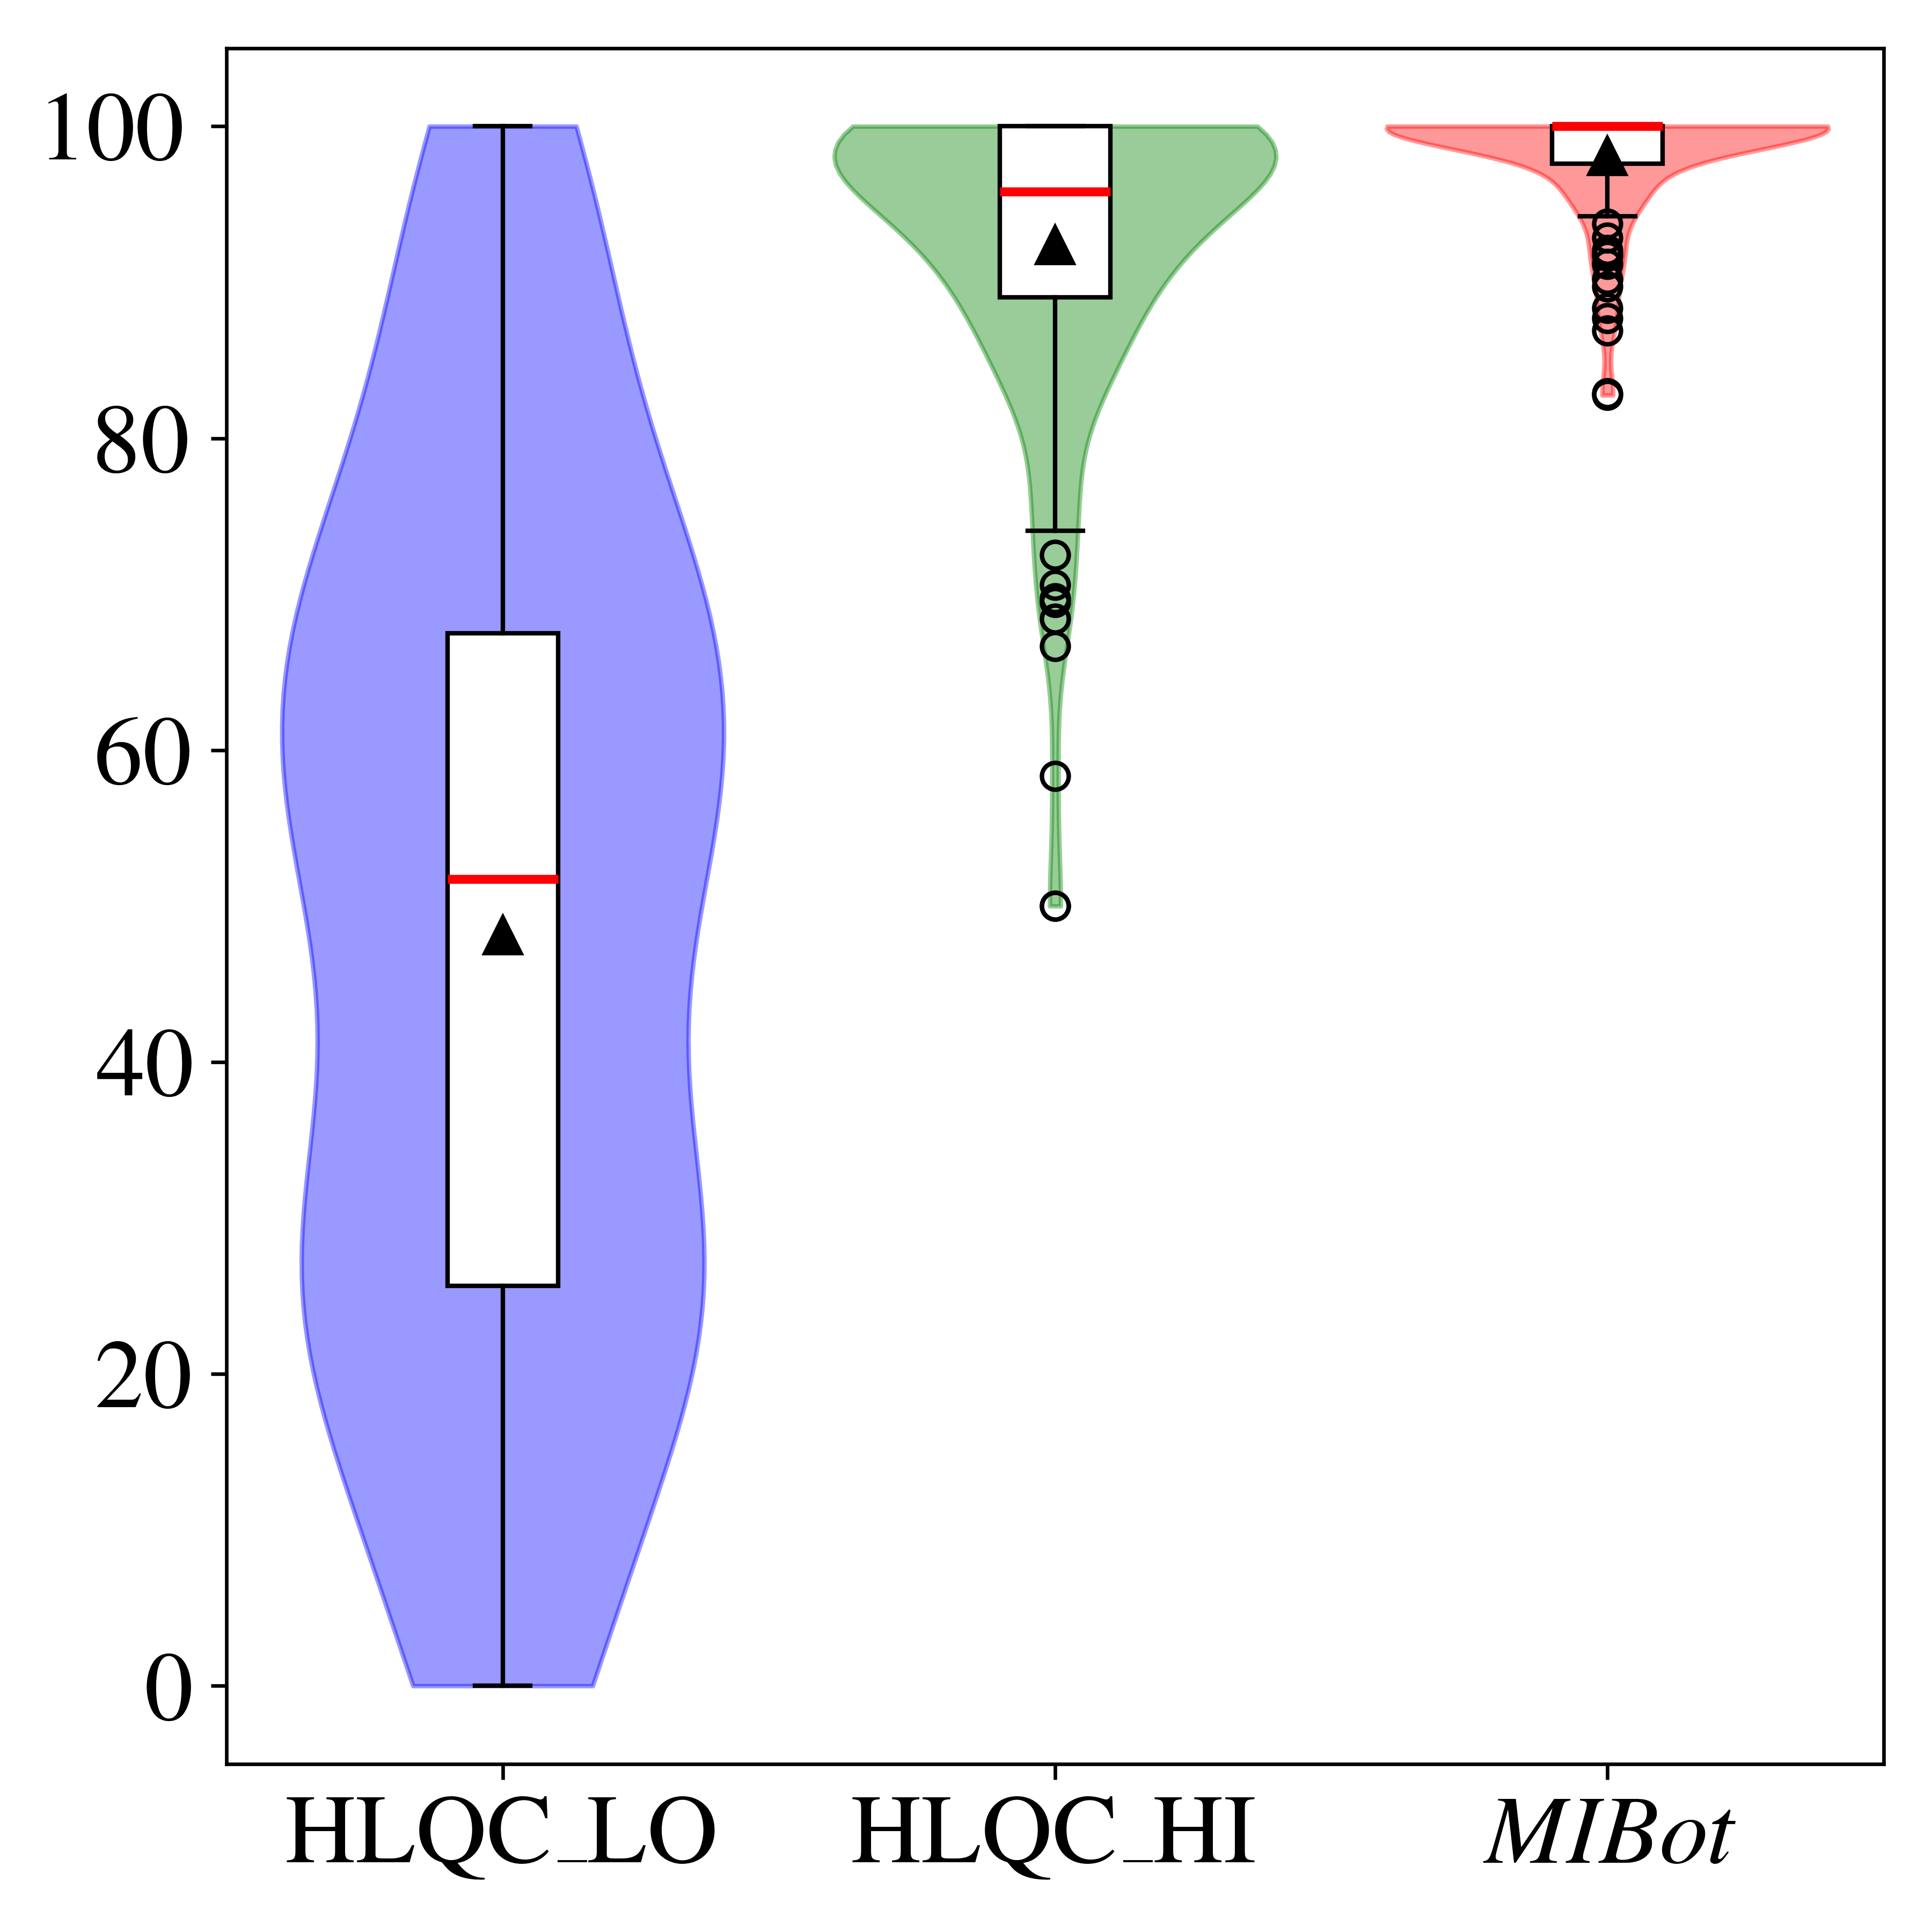
\includegraphics[width=\textwidth]{fig/mic.png}
        \caption{Percentage MI-Consistent Responses\\(\%MIC)}
        \label{fig:mic}
    \end{subfigure}
    \hfill
    \begin{subfigure}[b]{0.32\textwidth}
        \centering
        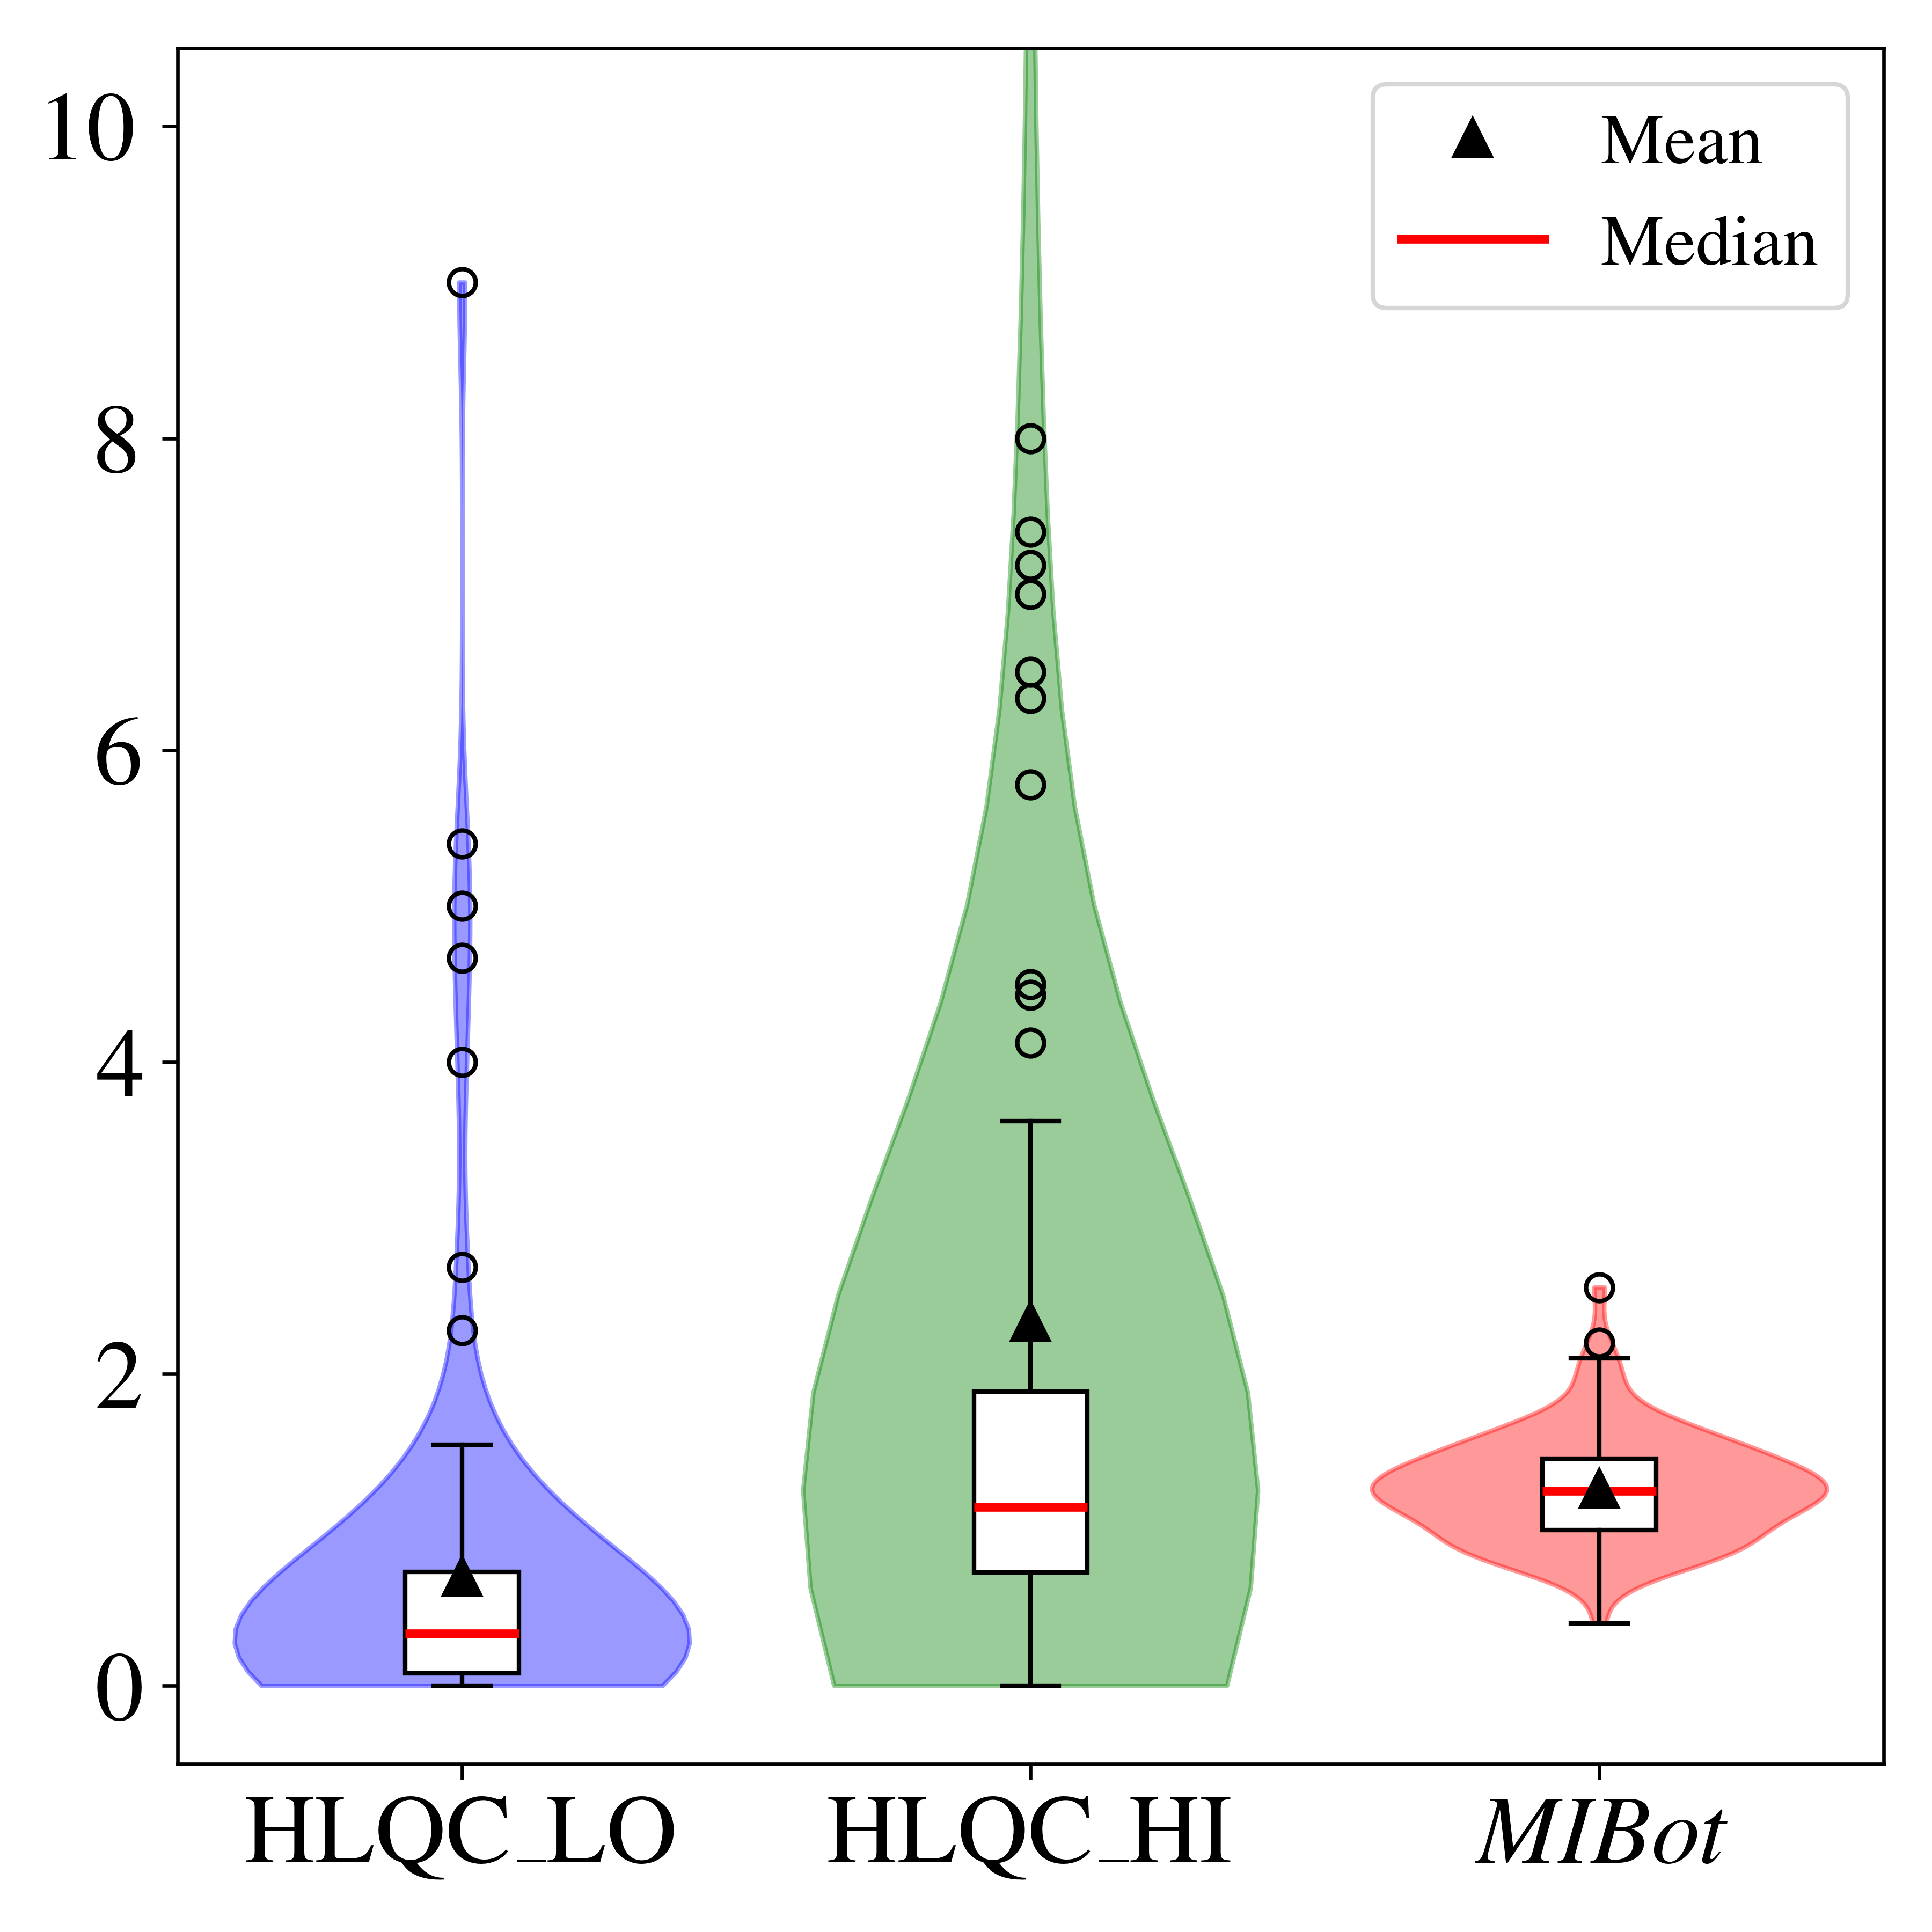
\includegraphics[width=\textwidth]{fig/rq.png}
        \caption{Reflection to Question Ratio \\(R:Q)}
        \label{fig:rq}
    \end{subfigure}
    \hfill
    \begin{subfigure}[b]{0.32\textwidth}
        \centering
        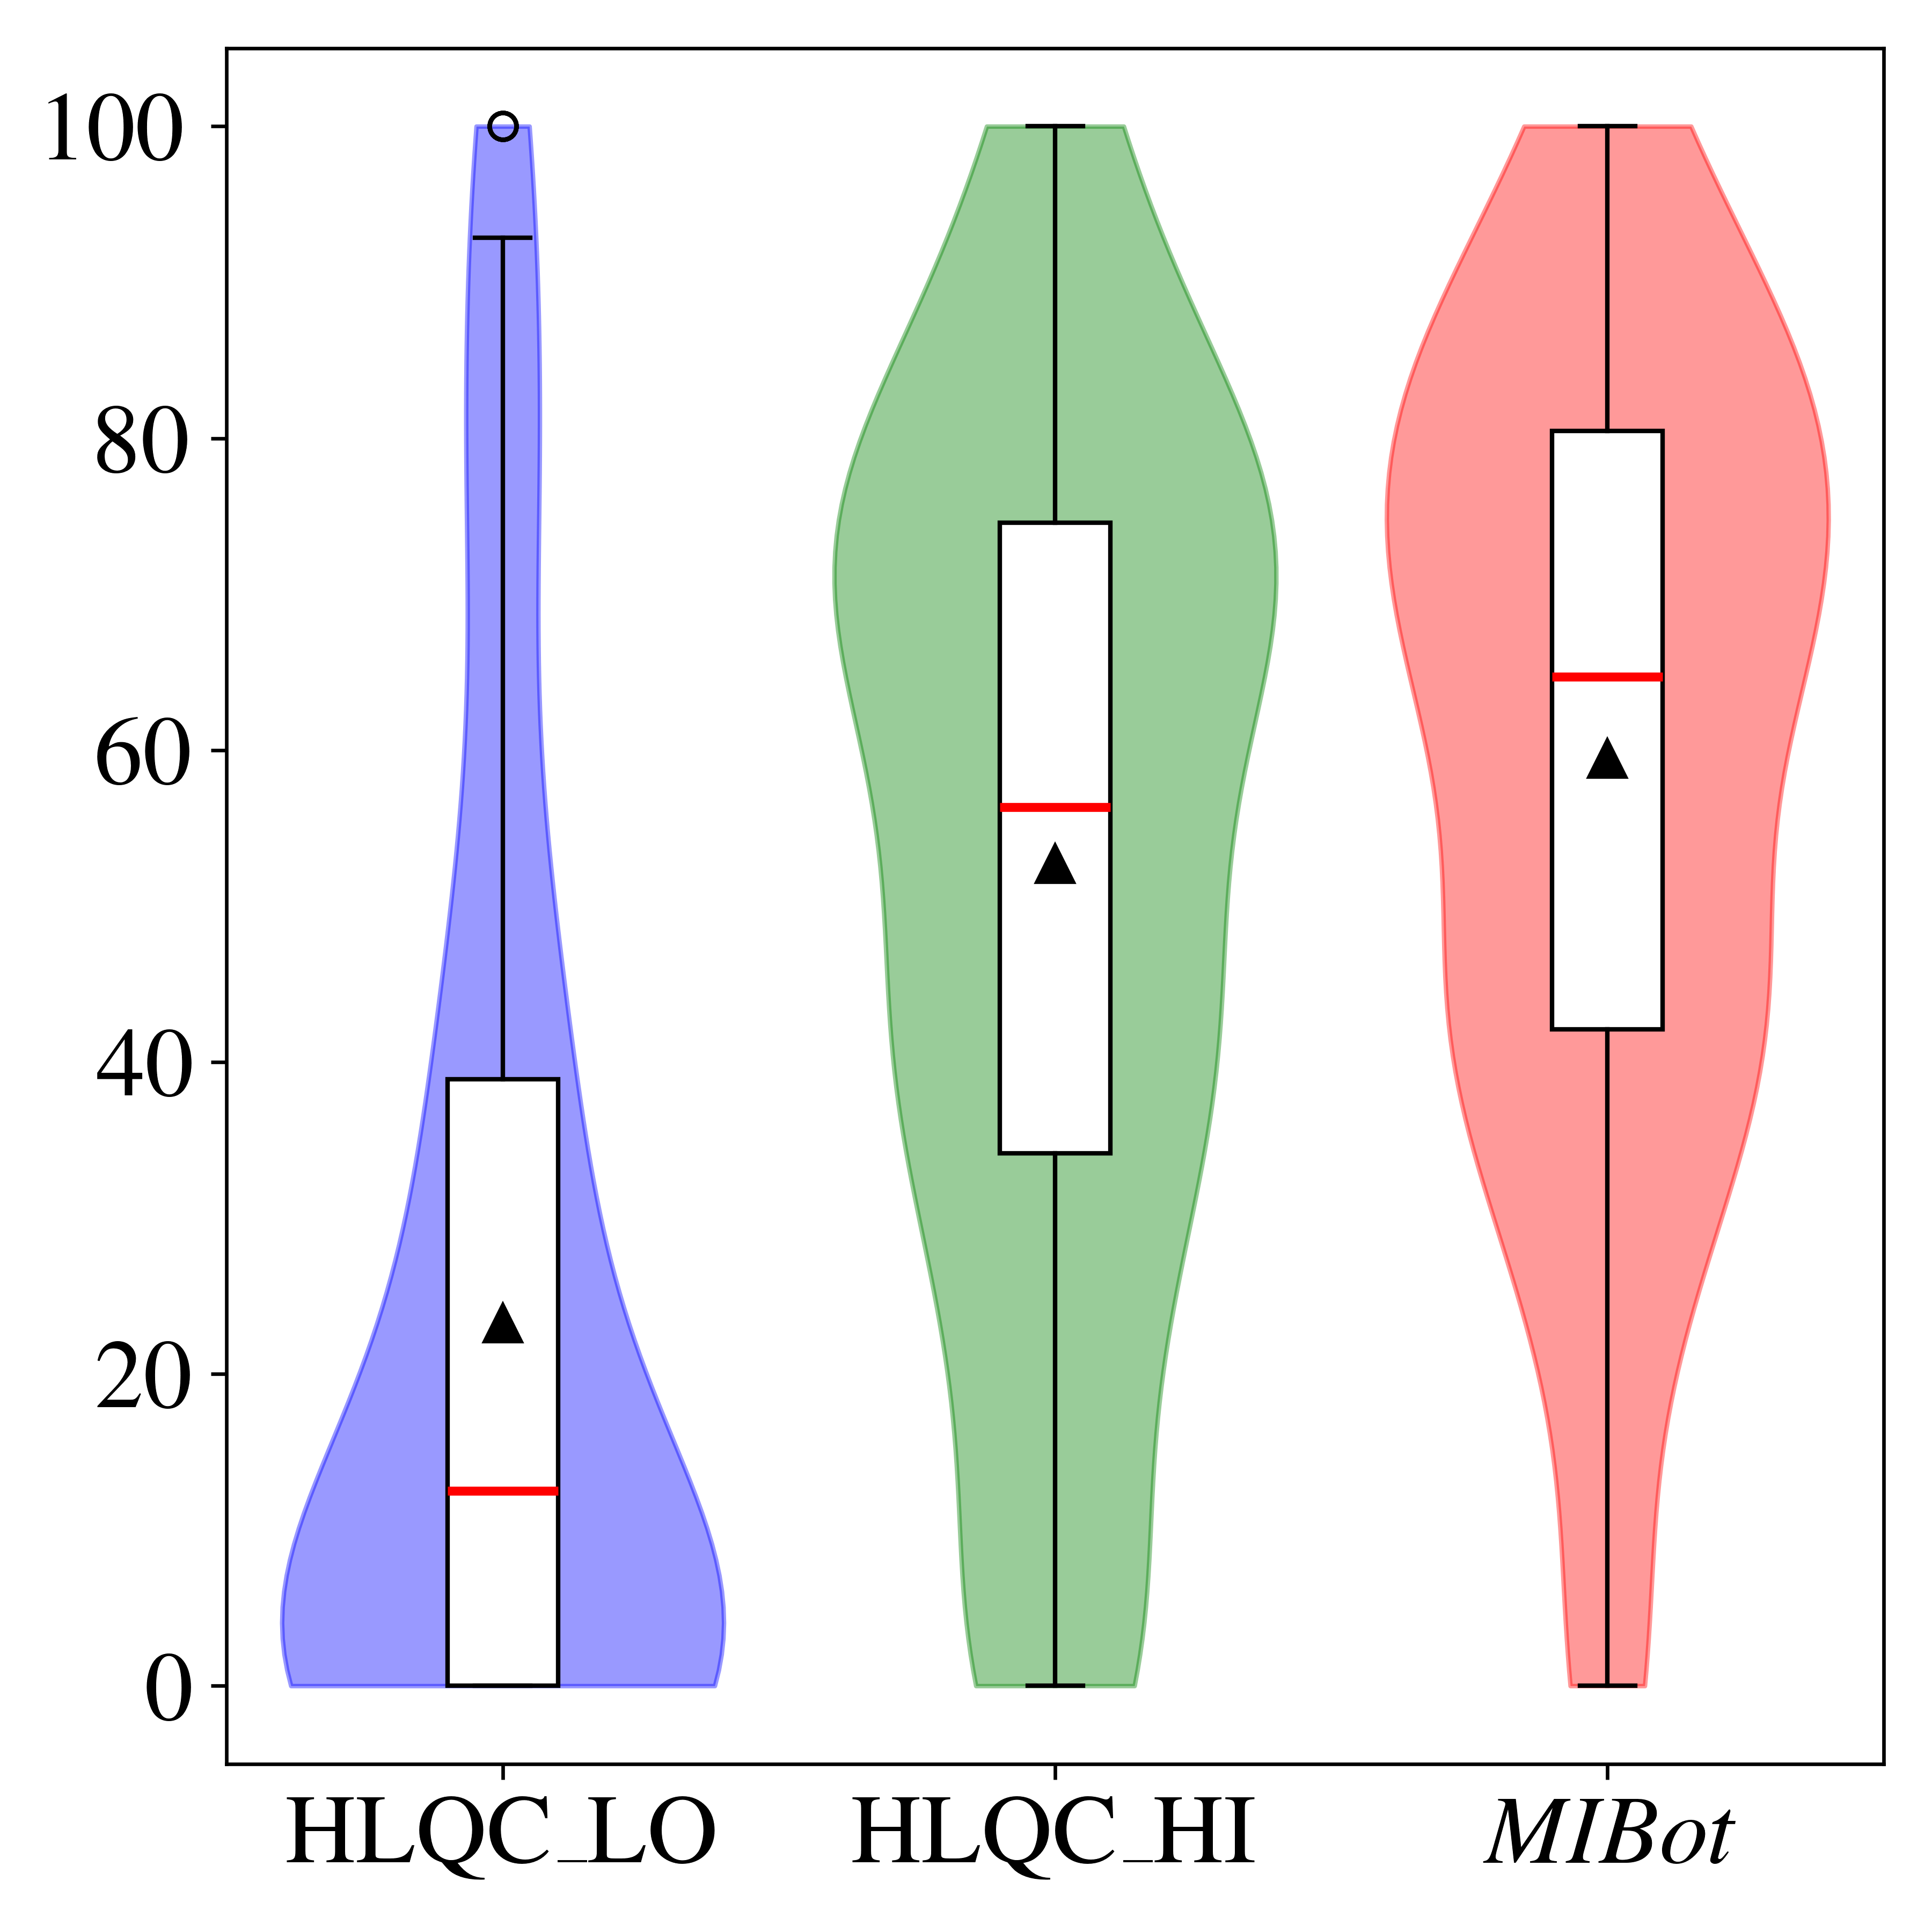
\includegraphics[width=\textwidth]{fig/ct.png}
        \caption{Percentage Client Change Talk \\(\%CT)}
        \label{fig:ct}
    \end{subfigure}
    \caption{Comparison of MISC summary score distributions across datasets.}
    \captionsetup{justification=justified}
    \label{fig:violin_box_plots}
\end{figure*}


\subsection{CARE Metric for Empathy}
\label{sec:CARE}
Each participant rated the perceived empathy of the chatbot on the CARE scale (\citealp{10.1093/fampra/cmh621}).
\textbf{Table~\ref{table:care}} presents the mean CARE scores for this work (\sysnamewithv) and our previous work, \oldsysname \citep{info:doi/10.2196/49132}. The fully generative \sysnamewithv is significantly more empathetic than a partially scripted and partially generative \oldsysname. Notably, 11\% of the participants gave \sysnamewithv a perfect score of 50, substantially higher than the 3\% achieved by \oldsysname. Compared to trained human counsellors, however, this number is quite low, as \citet{Bikker2015} found that nurses scored an average of 46 on the CARE metric, with 48\% achieving a perfect score of 50.
\begin{table}[htpb]
  \centering
  \setlength{\tabcolsep}{3pt}
  \renewcommand{\arraystretch}{0.9}
   {
  \begin{tabular}{@{}l@{\hspace*{3mm}}rr@{}}
    \toprule
    \textbf{} & \textbf{CARE} & \textbf{\% Perfect} \\
    \textbf{} & \textbf{Score} & \textbf{Score} \\
    \specialrule{0.4pt}{1pt}{1pt}
    \oldsysname & 36 & 3 \\
    \sysnamewithv & 42  & 11 \\
    Humans$^*$  & \textbf{46} & \textbf{48} \\
    \bottomrule
  \end{tabular}}
  \caption{Average CARE scores and (\%) perfect scores for \oldsysname, \sysnamewithv (present work) and $^*$typical human healthcare professionals \citep{Bikker2015}.
  }
  \label{table:care}
\end{table}


Appendix~\ref{appendix:CAREdist} provides the distribution of CARE scores among participants and question-wise mean CARE scores. The chatbot performed poorly on questions, such as ``How well did the chatbot show interest in you as a whole person?'' and ``How well did it assist in making a plan of action with you?''. The poor performance on some questions may be due to the chatbot's lack of emotional intelligence \citep{sabour-etal-2024-emobench} or collaboration skills \citep{yang-etal-2024-human}.

The general post-conversation survey showed that 92\% of participants enjoyed the experience, while 66\% found the interactions helpful.

\subsection{Adherence to MI}
\label{misc_summary_metrics}

The AutoMISC assessment tool, described in Section~\ref{sec:automisc_val}, was applied to the 106 transcripts from the study. To provide a point of comparison for the MISC summary metrics, we also ran it on the \textbf{High\-Low\-Quality\-Counselling (HLQC)} dataset \cite{perez-rosas-etal-2019-makes}, a publicly available\footnote{ \url{https://lit.eecs.umich.edu/downloads.html}} corpus of transcribed MI counselling demonstrations. It was designed to support the development of  ``data-driven methods for the automatic evaluation of counselling quality.'' The HLQC dataset comprises 155 high-quality (HLQC\_HI) and 104 low-quality (HLQC\_LO) transcripts sourced from public websites. We computed summary scores separately for these subsets and then compared \sysname's summary metrics against those of both HLQC\_HI and HLQC\_LO. \textbf{Table~\ref{table:mi_metrics_summary}} summarizes the computed MISC metrics across datasets. It shows that a very high fraction of the chatbot counsellor utterances are MI-compliant (\%MIC in the table), exceeding those in the high-quality dataset with less variance. The chatbot's Reflection to Question Ratio (R:Q) falls between that of the high- and low-quality datasets and aligns with the 1-2 range recommended in the MISC rubric. Finally, the fraction of participant utterances classified as \textit{change talk} is higher than in the high-quality dataset.


\begin{table}[thpb!]
  \centering
  \setlength{\tabcolsep}{4pt}
  \renewcommand{\arraystretch}{0.9}
  {
  \begin{tabular}{@{}llr@{}}
    \toprule
    \textbf{Metric} & \textbf{Dataset} & \textbf{Mean (SD)} \\
    \specialrule{0.4pt}{1pt}{1pt}

    \multirow{3}{*}{\textbf{\%MIC}}
    & HLQC\_LO & 48 (27.9) \\
    & HLQC\_HI & 92 (9.8) \\
    & \sysname & \textbf{98 (3.6)} \\

    \arrayrulecolor{gray!50}\midrule\vspace{-4pt}\\[-8pt]

    \multirow{3}{*}{\textbf{R:Q}}
    & HLQC\_LO & 0.7 (1.3) \\
    & HLQC\_HI & \textbf{2.3} (5.7) \\
    & \sysname & 1.3 \textbf{(0.3)} \\

    \arrayrulecolor{gray!50}\midrule\vspace{-4pt}\\[-8pt]

    \multirow{3}{*}{\textbf{\%CT}}
    & HLQC\_LO & 23 (29.5) \\
    & HLQC\_HI & 53 (28.4) \\
    & \sysname & \textbf{59 (25.6)} \\

    \arrayrulecolor{black}\bottomrule
  \end{tabular}}
  \caption{Comparison of MISC summary metrics in present study and the HLQC Datasets.}
  \label{table:mi_metrics_summary}
\end{table}


\textbf{Figures \ref{fig:mic}} and \textbf{\ref{fig:rq}} show the distribution, in violin plots, of counsellor's Percentage MI-Consistency (\%MIC) and Reflection-to-Question Ratio (R:Q) for the three datasets (HLQC\_LO, HLQC\_HI, \sysname). \sysname's distribution of \%MIC scores closely matches those of HLQC\_HI, another indication that the conversation adhered to the principles of MI. The R:Q distribution has a similar behaviour.


\textbf{Figure~\ref{fig:ct}} shows the violin plot distribution of the \% Client Change Talk (\%CT). The distributions for \sysname and HLQC\_HI are very similar, as were the averages. This is perhaps the most important indication of the \sysname's effectiveness ---  cultivating change talk is the key goal in MI.


\subsection{Dataset Release}
\label{dataset_release}
We are releasing most of the data collected in this study, including the transcripts of the conversation between the chatbot and participants, the Auto\-MISC annotations for both counsellor and client utterances, and summary metrics. For each participant, the dataset also includes their readiness ruler survey responses, CARE survey, \emph{Heaviness of Smoking} survey \citep{heatherton1989measuring}, and the feedback they provided on the conversation. This is described in more detail in Appendix~\ref{appendix:dataset_overview}.

Several studies have published MI counselling datasets \citep{perez-rosas-etal-2019-makes,welivita-pu-2022-curating,cohen-etal-2024-motivational,sun-etal-2024-eliciting,younsi-etal-2024-beyond}, but none have employed self-reported metrics or well-established surveys to measure the effectiveness of counselling. Our dataset is the first attempt in this direction, as it provides a holistic view of automated MI and its effectiveness on humans.